\documentclass[12pt]{beamer}
%% USE PACKAGES
\usepackage{amsfonts, amsmath, amssymb, array}
\usepackage{calc, cancel, caption, color}
\usepackage{datatool, dirtree}
\usepackage{etoolbox}
\usepackage{fancyhdr}
\usepackage{graphicx}
\usepackage{hyperref}
\usepackage{import}
\usepackage[utf8]{inputenc}
\usepackage{lipsum, listings, longtable}
\usepackage{multicol, marginnote}
%\usepackage{natbib}
\usepackage{parskip, perpage, pgfplots} %the perpage package
\usepackage{ragged2e, relsize}
\usepackage{scalefnt, stackengine}
\usepackage{textcomp, tikz}
\usepackage{url}
\usepackage{varioref}
\hypersetup{ colorlinks,citecolor=black,filecolor=black,linkcolor=black,urlcolor=black}
%% MACROS
\AtBeginSection[]
{
  \begin{frame}{Outline}
    \tableofcontents[currentsection,hideothersubsections]
  \end{frame}
}

\DeclareMathOperator*{\argmin}{arg\,min}
\DeclareMathOperator*{\argmax}{arg\,max}

%% LSTSET
\lstset{
	language=c++,
  	frame=single,
  	framesep=\fboxsep,
  	framerule=\fboxrule,
  	rulecolor=\color{black},
  	xleftmargin=\dimexpr\fboxsep+\fboxrule,
  	xrightmargin=\dimexpr\fboxsep+\fboxrule,
  	breaklines=true,
  	basicstyle=\small\ttfamily, % Global Code Style
  	identifierstyle=\color{black},
  	commentstyle=\color{eclipseGreen},
  	numbers=left, % show line numbers at the left
  	numberstyle=\small\ttfamily, % style of the line numbers
  	backgroundcolor=\color{black!7},
  	tabsize=2,
  	columns=flexible,
  	keywordstyle={\ttfamily\color{blue!90!black}},
  	morekeywords={vec3},
	keywords=[4]{Monster,Monsters},
	keywords=[5]{10},
	keywordstyle={[4]\color{orange!60!black}},
}

%% CAPTION SETUP
\captionsetup[lstlisting]{labelfont=bf,labelsep=period,calcwidth=1\linewidth,font=footnotesize}
\captionsetup[figure]{labelfont=sf,hypcap=false,format=hang,margin=1cm,justification=RaggedRight,calcwidth=0.8\linewidth,font=footnotesize,justification=justified}
\captionsetup[table]{labelfont=sf,hypcap=false,format=hang,margin=1cm,justification=RaggedRight,calcwidth=0.8\linewidth,font=footnotesize,justification=justified}


%% TIKZ
\usetikzlibrary{shapes.geometric, arrows,matrix, fit, patterns}
\usetikzlibrary{positioning}
\usetikzlibrary{decorations.text}
\usetikzlibrary{decorations.pathmorphing}
\pgfdeclarelayer{background}
\pgfsetlayers{background,main}
\pgfplotsset{compat=1.12}
\tikzstyle{startstop} 		= [rectangle,  rounded corners,minimum width=4cm, minimum height=1cm, text centered, draw=black, fill=red!30]
\tikzstyle{process}   		= [rectangle, minimum width=4cm, minimum height=1cm, text centered, draw=black, fill=orange!30]
\tikzstyle{optionalprocess} = [rectangle, minimum width=4cm, minimum height=1cm, text centered, draw=black, fill=orange!30, dashed]
\tikzstyle{io} 				= [trapezium, trapezium left angle=70, trapezium right angle=110, minimum width=3cm, minimum height=1cm, text centered, draw=black, fill=blue!30]
\tikzstyle{arrow} = [thick,->,>=stealth]



%% GENERAL USEFUL
\usepackage{array}
\newcolumntype{L}[1]{>{\raggedright}m{#1}}
\newcolumntype{C}[1]{>{\centering}m{#1}}
\newcolumntype{R}[1]{>{\raggedleft}m{#1}}


%%%%%%%%%%%% 
% Template %
%%%%%%%%%%%%
% Page dimension
\paperwidth=19cm
\paperheight=12cm
\textwidth=17cm
\oddsidemargin=-1.5cm
\topmargin=0cm
\headsep=5pt
\marginparsep=0.3cm
\marginparwidth=1cm
\voffset=-1.75cm
\hoffset=0cm

%Header
\def\title#1{\gdef\@title{#1}\gdef\stored@title{#1}}
\setbeamertemplate{navigation symbols}{}
\pagestyle{fancy}
\fancyhf{}
\lhead{\footnotesize\textbf{Örebro University}\hspace{10pt}{\scriptsize School of Science and Technology - \@title}}
\rhead{\scriptsize\thepage}
\renewcommand{\headrulewidth}{0pt}

% Footer
\lfoot{\scriptsize\today}
\cfoot{\scriptsize \insertsection}
\renewcommand{\sectionmark}[1]{\markright{\thesection\ #1}}
\rfoot{\fancyplain{}{ \scriptsize\textcopyright\hspace{3pt}  Benny Frost, Tom Olsson }}
% Title frame
\fancypagestyle{fancyonlheadings}{
\renewcommand{\headrulewidth}{0pt}
\lhead{\scriptsize Örebro Unversity\\
\textbf{School of Science and Technology}}
\lfoot{\scriptsize\today}
\rhead{}
}


\bibliographystyle{ieeetr}
% Title data
\title{Project: Differential Drive via WiFi}
\subtitle{Project presentation}
\author{Benny Frost, Tom Olsson}
\date{\today}
\institute{Örebro University}

\setbeamertemplate{section in toc}[sections numbered]
\setbeamertemplate{subsection in toc}[subsections numbered]


%%%%%%%%%%%%%%%%% 
% Last settings %
%%%%%%%%%%%%%%%%%
\begin{document}


%In beamer, these changes have no effect in preamble
\textheight=10cm
\headheight=0.5cm
\footskip=5pt


%%%%%%%%%
% Title %
%%%%%%%%%
% Title template
\defbeamertemplate*{title page}{customized}[1][]{
\thispagestyle{fancyonlheadings}
\large{\textbf{Örebro University}}\\\vspace{10pt}
{\usebeamercolor[fg]{title}\Huge\@title}\\\vspace{2cm}
{\Large\insertsubtitle}\\\vfill\vspace{2cm}
{\Large\insertauthor}\par
{\Large\insertinstitute}\\\vspace{0.5cm}
{\small\today \hspace{\fill} \textcopyright\hspace{3pt}  Benny Frost, Tom Olsson }
}



\maketitle
\section{Project}


\begin{frame}{Project definition}
\begin{itemize}
\item<1-> Build a robot with two motors
\item<2-> Setup the two motors, along with a differential drive controller
\item<3-> Add WiFi communication instead of serial
\item<4-> Calibrate the odometry
\end{itemize}
\onslide<5-> Hardware: Arduino Due \cite{arduinodue}, Motor Shield rev. 3 \cite{motorshield}, WiFi Shield \cite{wifishield}
\end{frame}

\section{Physical design}
\begin{frame}{Building the robot}
  \begin{itemize}
  \item<+-> Main body built from aluminum plating and profiles
    \item<+-> Details primarily built from plexiglass
  \item<+-> Two driving front wheels
    
  \item<+-> First design:
  \begin{itemize}
  \item<+-> Two slippery/smooth rear wheels
  \item<+->[$\Rightarrow$] Motors too weak to force the sliding
    
  \end{itemize}
  \item<+-> Second design:
  \begin{itemize}
  \item<+-> One centered swivel wheel at the rear
    \item<+->[$\Rightarrow$] Much better performance, but some issues because of the swivel (shopping cart syndrome)
  \end{itemize}
  \end{itemize}
\end{frame}

\begin{frame}{Motors \& power}
  \begin{itemize}
  \item<+-> The same motor shield as for laboration one was used, the Motor Shield Rev. 3 \cite{motorshield}
  \item<+-> The shield can handle up to 18 V input, and output 2 A per channel, but this requires the Arduino power circuits (3.3 V, 5 V and \emph{vin}) to be completely separated from the motor power supply
  \item<+-> To supply it with power, we created a battery pack with 12 AA batteries in series, which supply 18 V total
  \item<+-> The pins on the Arduino main board that were needed for the WiFi card were moved to other pins
    \item<+-> Similarly, the main Arduino board was battery powered by a 9 V battery
  \end{itemize}
  \end{frame}
\section{Motor setup and tuning}
\begin{frame}{Tuning \& setup}
  \begin{itemize}
  \item<+-> Two different PID-setups, one for each motor
  \item<+-> One big problem to solve:
    \begin{itemize}
       \item<+-> The motors have a large (but different) deadband where it doesn't move
      \item<+->[$\Rightarrow$] The deadband roughly in the range $\left[0,700\right]$, but one motor is slightly easier to start
   \end{itemize}
 \item<+-> To reduce the impact of the deadband, all actuation values from 10 to 700 were set to 700, and all below 10 were set to 0
   \item<+-> We also added feedback in the PID controller, so that some of the current output PWM is counted as ``promised speed'', which smoothes the PID output by approximating the smoothing applied to the velocity reading
  \end{itemize}
  
\end{frame}


\begin{frame}{Adding the WiFi communication}
\begin{itemize}
\item<+-> The \texttt{ros\_lib} \textbf{\texttt{NodeHandle}} is a template class, and accepts a \texttt{Stream} interface object as the template argument
\item<+-> This is normally a \texttt{Serial} class reference
\item<+-> However, the \texttt{\textbf{WiFi}} module is also a derivative of \texttt{Stream}
\item<+-> Therefore, it should be relatively easy to change between the two classes  
\begin{itemize}
	\item<+-> Replace references to \texttt{Serial} with \texttt{WifiClient}
	\item<+-> Add connection management code
	\item<+-> \emph{Done?}
\end{itemize}
\end{itemize}
\end{frame}

\begin{frame}{Arduino WiFi}
  \begin{itemize}
  \item<+-> The official WiFi shield from Arduino \cite{wifishield}
  \item<+-> In order to connect it to the main board some pins had to be rewired, as some are used by both the Motor shield and the WiFi shield
  \item<+-> Comes with several drawbacks that we discovered on our own and verified with other sources:
    \begin{itemize}
    \item<+-> Has a 2-second cycle rate for transmitting - in practice, it only sends packages once every other second
    \item<+-> Has a maximum message size of 92 bytes for each call to the shield firmware - a limitation in the SPI bus
    \item<+-> Will silently fail on any overflow in any buffer \cite{wificard1, wificard2}
    \end{itemize}
    \item<+-> Because of these problems, eventually we replaced the WiFi shield with an ESP8266 microcontroller as WiFi card
  \end{itemize}
\end{frame}
\begin{frame}{ESP8266}
  \begin{itemize}
    \item<+-> The ESP8266 is a standalone microcontroller with built-in WiFi \cite{ESP8266}
    \item<+-> This card is often recommended instead of the official WiFi card both because of its cost as well as good performance
    \item<+-> Has its own toolchain, and runs the code on its own in a separate process from the main Arduino board \textbf{asynchronously}
    \item<+-> In this case, it is used like a router, only relaying information between two communicating devices
  \end{itemize}
\end{frame}
\begin{frame}{Communication}
	\begin{figure}[h]
		\resizebox{1\linewidth}{!}{
			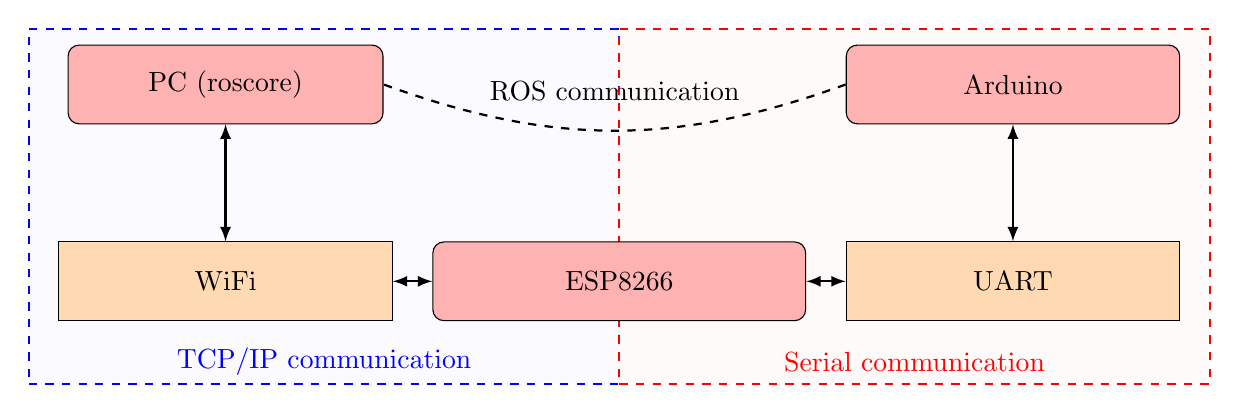
\begin{tikzpicture}[node distance=2cm]
				\begin{pgfonlayer}{main}
				\node (pc) [startstop] {PC (roscore)};
				\node (serial) [process, below of=pc,yshift=-0.5cm, text width=4cm] {WiFi};
				\node (esp) [startstop, right of=serial,xshift=3cm,text width=4.5cm] {ESP8266};
				\node (deserialize) [process, right of=esp,xshift=3cm,text width=4cm] {UART};
				\node (arduino) [startstop, above of=deserialize,yshift=0.5cm, text width=4cm] {Arduino};
				
				\draw [latex-latex,thick] (pc) -- (serial) node [midway, left] (TextNode) {};
				\draw [latex-latex,thick] (serial) -- (esp) node [midway, left] (TextNode) {};
				\draw [latex-latex,thick] (esp) -- (deserialize) node [midway, left] (TextNode) {};
				\draw [latex-latex,thick] (deserialize) -- (arduino) node [midway, left] (TextNode) {}; 
				\draw [dashed,thick] (arduino.west) to[bend left=20] node[midway, above,yshift=0.5cm, anchor=center] (TextNode) {ROS communication}  (pc.east);
				\end{pgfonlayer}
\begin{pgfonlayer}{background}
				\node (kd) [draw=blue, fit=(pc) (serial) (esp), inner sep=0.15	cm, inner ysep=0.5cm, yshift=-0.3cm, xshift=-1.375cm, inner xsep=-1cm, dashed, thick, fill=blue!10, fill opacity=0.2] {};
				\node [yshift=2ex, blue] at (kd.south) {TCP/IP communication};
				
				\node (kd) [draw=red, fit=(deserialize) (arduino) (esp), inner sep=0.15cm, inner ysep=0.5cm, yshift=-0.3cm, xshift=1.375cm, inner xsep=-1cm, dashed,  thick, fill=red!10, fill opacity=0.2] {};
				\node [yshift=2ex, red] at (kd.south) {Serial communication};
\end{pgfonlayer}
			\end{tikzpicture}
		}
		\captionof{figure}{System view of communication}\label{tikz:communication}
	\end{figure}
\end{frame}
\begin{frame}{PC setup}
\begin{itemize}
\item<+-> The PC runs the \texttt{roscore} for the system
\item<+-> Two nodes are used on the PC to control the robot:
\begin{itemize}
\item<+-> \texttt{rosserial\_python} in TCP/IP mode to handle communication and serialization
\item<+-> a Python script for sending command messages to the robot\\(\texttt{geometry\_msgs::Twist}). This script comes from Husqvarna and is intended for\\research with their robotic mower
\end{itemize}
\end{itemize}
\end{frame}
\begin{frame}{ESP8266 setup}
\begin{itemize}
\item<+-> The ESP8266 is set up to be a very basic passthrough module
\item<+-> It does two things:
\begin{itemize}
\item<+-> Read from WiFi, write to Serial
\item<+-> Read from Serial, write to WiFi
\end{itemize}
\item<+-> It also makes sure that the WiFi connection is maintained
\end{itemize}
\end{frame}
\begin{frame}{Arduino setup}
\begin{itemize}
\item<+-> The Arduino module is almost the same as laboration 1, but is a differential drive controller instead of a basic velocity controller
\item<+-> Three changes were made:
\begin{itemize}
\item<+-> Reduce the serial bus speed by 25 \% down to 38.4k
\item<+-> Add a ``retry'' for delayed bytes allowing up to 20ms of packet delays
\item<+-> Use Serial1 (TX1,RX1) instead of Serial/USB (TX0,RX0)
\end{itemize}
\item<+-> And as mentioned before, a feedback term was added to the PID controller
\end{itemize}
\end{frame}
\begin{frame}{Reason for changes: protocol mismatch}
\begin{minipage}[t]{.45\linewidth}%
  {\onslide<1-> \large\textbf{TCP/IP}}\\
  \begin{itemize}
    
\item<2->[$\bullet$] Guaranteed delivery, but not in order and not at specific time point
\item<3->[$\bullet$] Varying speed
\item<4->[$\bullet$] Any packet size
\end{itemize}
\end{minipage}\hspace{1cm}\begin{minipage}[t]{.45\linewidth}%
  {\onslide<1-> \large\textbf{Serial}}\\
  \begin{itemize}
\item<2->[$\bullet$] Guaranteed order and specific time-point
\item<3->[$\bullet$] Fixed speed (baud rate) 
\item<4->[$\bullet$] Fixed packet size
\end{itemize}
\vspace{.5cm}
\end{minipage}
\begin{itemize}
\item<5->[$\Rightarrow$] These do not match very well, which causes synchronization problems
\item<6->[$\Rightarrow$] Generally because the Serial is too fast for the WiFi communication
\item<7->[$\Rightarrow$] This causes the Arduino to receive "empty" from the Serial bus, while the ESP8266 is still processing parts of the message from the WiFi connection
\item<8->[$\Rightarrow$] When reading empty, the Arduino will (by default) drop the message entirely and ask for a resynchronization... which will fail too
  \end{itemize}
\end{frame}
\begin{frame}{Odometry measurements}
  \begin{itemize}
  \item<+-> Very random behaviour; and very inaccurate when doing ``goto'' commands. These were added as an afterthought, and this may affect their performance.
  \item<+-> The rear wheel has serious problems with movement and will often get stuck at odd angles causing the robot to drift
  \item<+-> Generally, the first line of a square will be perfectly straight, and then after the first turn it will keep turning slightly without $\theta$ reflecting this
  \item<+-> However, when manually controlling the robot and sending velocity commands it is much easier to get accurate readings
    \item<+-> By doing this, it is easy to see that the error is introduced each time a turn is made, and that this error is caused by the swivel wheel going the wrong way when starting to move forward after the turn
  \end{itemize}
\end{frame}
{ \smaller
  \bibliography{references}
  }
\end{document}

%%% Local Variables:
%%% mode: latex
%%% TeX-master: t
%%% End:
